\subsubsection{Notation}
\label{FullNotation}
J.G. Walker developed a notation to define these constellations with only 4 parameters \cite{Walker1977}:

\begin{equation*}
i: T/P/F
\end{equation*}
\begin{itemize}
\item i: inclination of the orbit in degrees
\item T: total number of satellites
\item P: number of planes
\item F: relative phase difference between satellites from adjacent planes
\end{itemize}

Since all satellites are placed at the same altitude, with these notation the shape of the pattern is completely determined. However, to determine all the orbital parameters it is necessary to know the radius of the orbits.

\subsubsection{Coverage}
\label{FullCoverage}
The previous section has shown that in polar orbits the coverage of the constellation could be determined with the streets of coverage method. On the other hand, in delta patterns it is necessary to study each configuration to verify its coverage. J.G. Walker determined that delta patterns gave better coverage than polar orbits, but not substantially better in the case of single coverage. This kind of patterns are more useful for double or triple coverage constellations, as it can be seen in Figure \ref{fig:Walker vs. polar}. However, his calculations were for a low number of satellites, so it is necessary to compute new results for the number of satellites of the Astrea constellation.

\begin{figure}[h]
\centerline{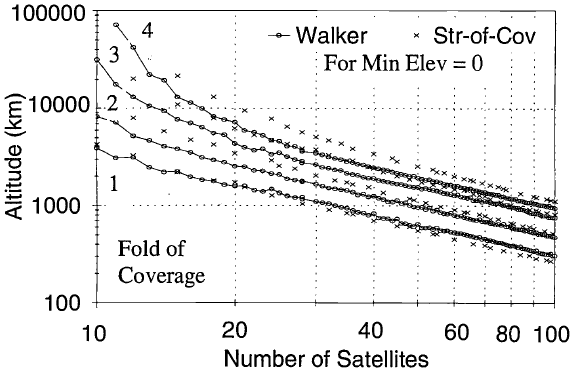
\includegraphics[scale=0.75]{foldofcoverage.png}}
\caption[Minimum altitude for continuous global coverage]{Minimum altitude for continuous global coverage. Comparison between polar patterns and Walker delta patterns. Extracted from \cite{Chobotov2002}}
\label{fig:Walker vs. polar}
\end{figure}